% Zadnja posodobitev: 14. 1. 2022
\documentclass[twoside,11pt]{article}
\usepackage[slovene]{babel}
\usepackage[utf8]{inputenc}
\usepackage{graphicx}
\usepackage[frame]{matrika}
\usepackage{mathtools}
\usepackage{epstopdf}
\usepackage{units}

% Po potrebi se lahk dodajo drugi standardni paketi, ki ne spreminjajo izgleda dokumenta
\usepackage{tikz}
\usepackage{amsmath}
\usepackage{float}
\providecommand{\set}[1]{\left\{#1\right\}}
\providecommand{\setb}[2]{\left\{#1~\middle\vert~#2\right\}}
\providecommand{\abs}[1]{\left\lvert #1\right\rvert}
\providecommand{\floor}[1]{\left\lfloor #1\right\rfloor}

\begin{document}
\MAT{1}{12}{2025}
\naslov{Ramseyeva teorija}

\avtor{Jan Pantner}

\institucija{Fakulteta za matematiko in fiziko \\ Univerza v Ljubljani}

\klasifikacija{05D10} 
\izvlecek{Članek obravnava osnovne pojme Ramseyeve teorije kot 
so Ramseyeva števila, grafovska Ramseyeva števila, Schurova števila in 
``The Happy End Problem''. Med drugim, dokaže Ramseyev izrek in nekaj zgornjih ter spodnjih mej za 
Ramseyevo število $R(r, s)$.}
\title{Ramsey theory}
\abstract{The article discusses the basic concepts of Ramsey theory, 
such as Ramsey numbers, graph Ramsey numbers, Schur numbers, and 
The Happy End Problem. Among other results, it proves Ramsey's theorem and presents some upper 
and lower bounds for the Ramsey number $R(r,s)$.}

\glava\baselineskip=14.5pt

\smallskip

\section{Uvod}

\hspace{\parindent}Ramseyeva teorija govori o particijah velikih struktur. Tipičen rezultat nam pove, da 
se mora v neki particiji dovolj velike strukture pojaviti neka specifična podstruktura. Na primer, 
če povezave dovolj velikega polnega grafa pobarvamo z nekaj barvami, mora nujno obstajati 
monokromatičen trikotnik (v tem primeru imamo particijo povezav na različne barve, 
osnovna struktura so povezave grafa, iskana podstruktura pa monokromatičen trikotnik).

Da zgornje res drži, nam zagotovi Ramseyev izrek, ki je nekakšna ``večdimenzionalna'' posplošitev 
Dirichletovega principa, ki tudi sam preučuje particije struktur (na primer razdelitev golobov v
golobnjake).

Bolj filozofsko, Ramseyeva teorija pove, da bodo ne gleda na to, kako kaotičen je nek sistem, 
znotraj sistema vedno obstajali urejeni deli.

Rezultati v članku so večinoma povzeti po \cite{color} in \cite{west}. V \cite{color} je 
predstavljeno tudi zgodovinsko ozadje razvoja Ramseyeve teorije.

\section{Osnovni rezultati}
\begin{zgled}
    Ali med poljubnimi šestimi ljudmi vedno obstajajo trije, ki se med seboj
    poznajo, ali trije, ki se med seboj ne poznajo?

    Poglejmo enega izmed teh ljudi. Brez škode za splošnost po Dirichletovem principu med 
    ostalimi petimi obstajajo trije, ki jih pozna. Če se poljubna dva med temi tremi poznata, 
    imamo tri ljudi, ki se med seboj poznajo. Sicer se ti trije med seboj ne poznajo, odgovor je 
    torej v obeh primerih pritrdilen.
\end{zgled}

Zgornji zgled je eden izmed enostavnejših rezultatov Ramseyeve teorije, vendar v nadaljevanju,
za lažje razumevanje, izjave raje formuliramo v jeziku teorije grafov in ne socialne interakcije.

Kot zanimivost lahko omenimo, da se Ramsey v 
resnici ni ukvarjal niti z grafi niti s socialnimi interakcijami, temveč z logiko. Izrek, po katerem 
je najbolj znan, je dokazal kot manjšo lemo na poti k popolnoma drugačnim rezultatom. Več 
o Ramseyu se nahaja v \cite[poglavje 30]{color}. Večina zgodnjega razvoja 
Ramseyeve teorije se je zgodila šele po njegovi smrti pri ranih $26$-tih letih. Za zgodnji razvoj je 
med drugimi v veliki meri zaslužen eden najznamenitejših matematikov 20.~stoletja 
Paul~Erdős.

\begin{izrek}[Ramsey] \label{izrek:ramseyosnovni}
    Za poljubni naravni števili $r$ in $s$ obstaja najmanjše takšno naravno število 
    $n = R(r,s)$, da velja naslednje: Če povezave polnega grafa $K_n$ pobarvamo z dvema barvama, 
    zagotovo obstaja poln podgraf moči $r$, v katerem so vse povezave prve barve, ali pa poln 
    podgraf moči $s$, v katerem so vse povezave druge barve.
\end{izrek}

Številu $R(r, s)$ pravimo \emph{Ramseyevo število}.
Iz definicije takoj sledi $R(r, s) = R(s, r)$ in $R(2, n) = n$.


Alternativna formulacija zgornjega izreka bi bila, da vsak graf na $n$ točkah vsebuje 
bodisi kliko moči $r$ bodisi antikliko moči $s$.
Dokaz te verzije izreka izpustimo, izrek \ref{izrek:ramsey} je splošnejši.


\begin{zgled}
    Določimo $R(3,3)$ in $R(3, 4)$.

    Pokazali smo že, da velja $R(3, 3) \le 6$ (ljudi predstavimo z vozlišči, poznanstva pa z barvo povezave). Za dokaz spodnje meje si poglejmo 
    sliko \ref{fig:r33}.
    Opazimo, da barvanje nima monokromatičnega trikotnika, torej $R(3, 3) > 5$. Skupaj smo dokazali 
    $R(3,3) = 6$.

    \begin{figure}[h!]
        \centering
        \newcommand\size{1}
        \begin{tikzpicture}[scale=2]
            \draw[thick,blue]  (18:\size) \foreach \a in {90,162,234,306} { -- (\a:\size) } -- cycle;
            \draw[thick,red] (18:\size) \foreach \a in {162,306,90,234} { -- (\a:\size) } -- cycle;
            \foreach \a in {18,90,162,234,306} { \node[black,fill=black,circle,inner sep=1.5pt] at (\a:\size){}; }
        \end{tikzpicture}
        \caption{Barvanje $K_{5}$ z dvema barvama, ki ne vsebuje monokromatičnega trikotnika.}
        \label{fig:r33}
    \end{figure}

    Slika \ref{fig:r34} prikazuje barvanje $K_{8}$ z rdečo in modro barvo, 
    ki nima rdečih trikotnikov in nima modrih klik velikosti $4$. Sledi $R(3, 4) > 8$. 
    \begin{figure}[h!]
        \centering
        \newcommand\size{1}
        \begin{tikzpicture}[scale=2]
            \draw[thick,blue]  (0:\size) \foreach \a in {0,45,90,135,180,225,270,315} { -- (\a:\size) } -- cycle;
            \draw[thick,blue]  (0:\size) \foreach \a in {0,90,180,270} { -- (\a:\size) } -- cycle;
            \draw[thick,blue]  (45:\size) \foreach \a in {45,135,225,315} { -- (\a:\size) } -- cycle;
            \draw[thick,red] (0:\size) \foreach \a in {0,135,270,45,180,315,90,225} { -- (\a:\size) } -- cycle;
            \draw[thick,red] (0:\size) \foreach \a in {0,180} { -- (\a:\size) } -- cycle;
            \draw[thick,red] (45:\size) \foreach \a in {45,225} { -- (\a:\size) } -- cycle;
            \draw[thick,red] (90:\size) \foreach \a in {90,270} { -- (\a:\size) } -- cycle;
            \draw[thick,red] (135:\size) \foreach \a in {135,315} { -- (\a:\size) } -- cycle;
            \foreach \a in {0,45,90,135,180,225,270,315} { \node[black,fill=black,circle,inner sep=1.5pt] at (\a:\size){}; }
        \end{tikzpicture}

        \caption{Barvanje $K_{8}$ z dvema barvama, ki ne vsebuje rdečega trikotnika ali 
        modre klike moči štiri.}
        \label{fig:r34}
    \end{figure}

    Pokažimo, da velja $R(3, 4) = 9$. Recimo, da imamo barvanje $K_9$ z rdečo in modro 
    barvo, ki ne vsebuje rdečega trikotnika in ne vsebuje modre klike moči štiri. Poglejmo 
    si neko vozlišče $v_0$. 
    \begin{itemize}
        \item Recimo, da je vozlišče $v_0$ vsebovano v vsaj šestih modrih povezavah. Zaradi 
        prejšnjega dela zgleda lahko med temi šestimi vozlišči najdemo tri vozlišča,
        ki tvorijo mmonokromatičen trikotnik. Če je slednji moder, skupaj z vozliščem $v_0$ tvori modro kliko moči 
        štiri, sicer pa imamo rdeč trikotnik.

        \item Recimo, da je vozlišče $v_0$ vsebovano v vsaj štirih rdečih povezavah. Če 
        med temi štirimi vozlišči (ki so z $v_0$ povezana z rdečo povezavo) ni nobene 
        rdeče povezave, tvorijo modro kliko moči štiri. Če obstajata med njimi vozlišči, 
        ki sta povezani z rdečo povezavo, tedaj skupaj z $v_0$ tvorita rdeč trikotnik.
    \end{itemize}
    
    Edina preostala možnost je, da je vsako vozlišče vsebovano v natanko treh rdečih povezavah. 
    V tem primeru podgraf, vpet na rdečih povezavah, krši lemo o rokovanju.
\end{zgled}

Eden izmed načinov, kako posplošiti Ramseyev izrek, je, da dodamo več barv. To prikazuje 
naslednji zgled. 

\begin{zgled}
    Določimo $R(3, 3, 3)$.
    Enostavno je pokazati $R(3,3,3) < 17$. Poglejmo vozlišče $v_0$. Brez škode za splošnost je vsebovano v vsaj šestih povezavah rdeče 
    barve. Če je med temi šestimi vozlišči kakšna povezava rdeče barve, smo končali, 
    sicer pa upoštevamo $R(3, 3) = 6$.

    Izkaže se, da velja enakost, torej $R(3, 3, 3) = 17$. Še več, obstajata natanko dve 
    neizomorfni barvanji grafa $K_{16}$, ki ne vsebujeta monokromatičnega trikotnika.
    Slika \ref{fig:r333} prikazuje enega od njiju.
    \begin{figure}[h!]
        \centering
        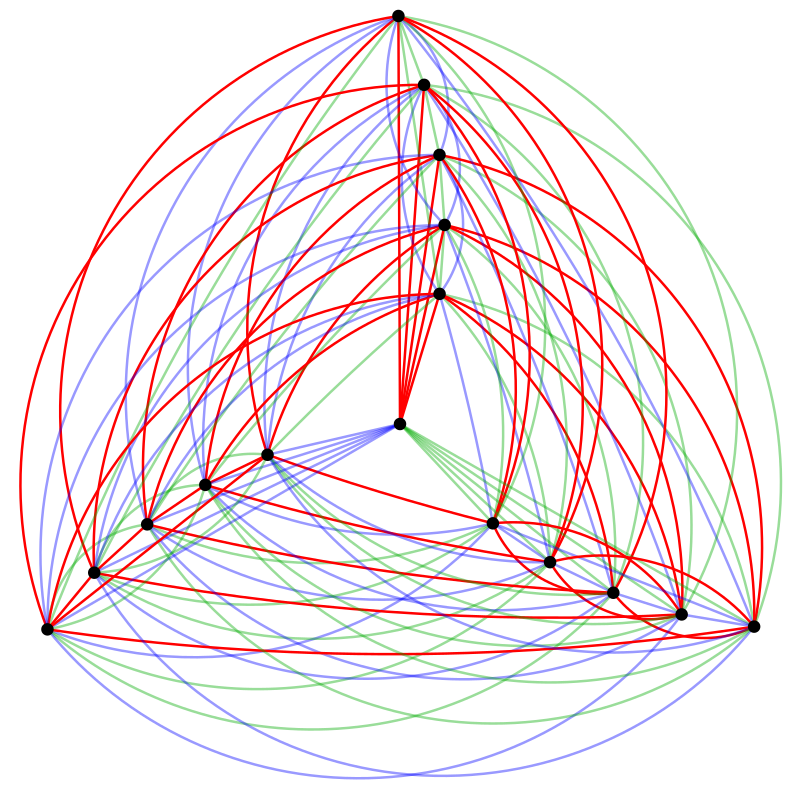
\includegraphics[scale=0.3]{r333.png}
        \caption{Barvanje $K_{16}$ s tremi barvanji, ki ne vsebuje monokromatičnega trikotnika. Vir: \cite{r333}}
        \label{fig:r333}
    \end{figure}
\end{zgled}

\section{Dokaz Ramseyevega izreka}

\begin{izrek}[Ramsey]
    Naj bo $r \ge 1$ in $a_1, a_2 \ge r$. Tedaj obstaja najmanjše takšno naravno število 
    $R(a_1, a_2; r)$, da velja naslednje: Če v množici $S$ moči $n \ge R(a_1, a_2; r)$
    vse $r$-podmnožice pobarvamo z barvo $1$ ali $2$, potem obstaja takšna $a_1$-podmnožica, 
    da so vse njene $r$-podmnožice barve $1$, ali pa obstaja takšna $a_2$-podmnožica, da so 
    vse njene $r$-podmnožice barve $2$. \label{izrek:ramsey}
\end{izrek}

\begin{dokaz}
    Uporabimo dvojno indukcijo, po $r$ in še po $a_1 + a_2$. 
    V primeru $r = 1$ velja $R(a_1, a_2; 1) = a_1 + a_2 -1$. Recimo, da je $a_1 \ge a_2$. Potem je 
    $R(a_1, a_2; a_2) = a_1$. Sedaj predpostavimo, da izrek velja za $r-1$ in ga dokažimo za $r$.
    Naj bo
    \begin{align*}
        a_1' &:= R(a_1 - 1, a_2; r), \\
        a_2' &:= R(a_1, a_2 -1; r).
    \end{align*}
    Naj bo $S$ množica moči več kot $R(a_1', a_2'; r-1) + 1$. Vse podmnožice $S$ pobarvamo z 
    barvo $1$ ali barvo $2$. Naj bo $a \in S$ in $S' := S \setminus \set{a}$. Barvanje $S'$ je 
    usklajeno z barvanjem $S$ tako, da je barva $X \subseteq S'$ enaka barvi $X \cap \set{a}$ v $S$.

    Ker velja $\abs{S'} \ge R(a_1', a_2';r-1)$, brez škode za splošnost obstaja $a_1'$-podmnožica $A$ 
    množice $S'$, v kateri so vse $(r-1)$-podmnožice barve $1$. Velja $\abs{A} = a' = R(a_1-1,a_2;r)$.
    Sedaj ločimo dva primera.
    \begin{itemize}
        \item Recimo, da v $A$ obstaja $a_2$-podmnožica, v kateri so vse $r$-podmnožice barve $2$.
        \item Recimo, da v $A$ obstaja $(a_1-1)$-podmnožica $A'$, v kateri so vse $r$-podmnožice barve $1$. 
        Tedaj definiramo
        \[
            A'' := A' \cap \set{a}.
        \]
        Velja $\abs{A''} = a_1$. Ker je barvanje $S' \supseteq A'$ usklajeno z barvanjem $S \supseteq A$, 
        so vse $r$ podmnožice v $A''$ barve $1$.
    \end{itemize}
    V obeh primerih smo izpolnili zahtevan pogoj, torej izrek velja tudi za $r$. \hfill $\blacksquare$
\end{dokaz}

V posebnem primeru $r = 2$ se izrek \ref{izrek:ramsey} zreducira 
na izrek \ref{izrek:ramseyosnovni}.

Naslednja trditev je zanimiv geometrijski rezultat, ki ga lahko dokažemo 
s pomočjo izreka \ref{izrek:ramsey}. 

\begin{izrek}[Erdős-Szekeres] \label{izrek:happyend}
    Za vsak $n \in \mathbb{N}$ obstaja tako število $N(n)$, da velja: Če imamo v ravnini $N \ge N(n)$
    točk v splošni legi, potem med njimi obstaja $n$ točk, ki določajo konveksen $n$-kotnik.
\end{izrek}

Najprej dokažimo naslednjo geometrijsko lemo.
\begin{lema}
    Množica $n$ točk v ravnini tvori konveksen $n$-kotnik natanko tedaj, kadar
    vsaka podmnožica štirih točk tvori konveksen $4$-kotnik.
\end{lema}
\begin{dokaz}
    Poglejmo konveksno ogrinjačo točk. Če točke tvorijo konveksen $n$-kotnik, potem vsake 
    štiri tvorijo konveksen štirikotnik. Nasprotno, recimo, da točke ne tvorijo konveksnega 
    $n$-kotnika. Potem obstaja točka znotraj ogrinjače. Če ogrinjačo trianguliramo, bo ta 
    točka znotraj nekega trikotnika in skupaj z oglišči trikotnika ne bo tvorila 
    konveksnega $4$-kotnika. \hfill $\blacksquare$
\end{dokaz}

\noindent\textit{Dokaz trditve.}
    Naj bo $N \ge N(n) := R(n,n;3)$. Točke označimo z $1, 2, \dots, N$. 
    Poglejmo poljuben trikotnik in njegova oglišča označimo z $i$, $j$, $k$ tako, da $i < j < k$. Če je 
    trikotnik $ijk$ pozitivno orientiran, ga pobarvamo s prvo barvo, sicer z drugo.

    Ker je $N \ge R(n,n;3)$, brez škode za splošnost obstaja $n$-podmnožica, v kateri so 
    vsi trikotniki prve barve. Dokažimo, da ta množica tvori konveksen $n$-kotnik. Predpostavimo 
    nasportno in uporabimo lemo. Torej obstajajo štiri točke, ki ne tvorijo konveksnega 
    štirikotnika. %Če pogledamo orientacije trikotnikov na teh štirih vozliščih, pridemo do 
    %protislovja s tem, da so vsi trikotniki iste barve. \hfill $\blacksquare$

    Naj bodo te štiri točke $i$, $j$, $k$ in $l$ -- kot jih prikazuje slika \ref{fig:happy}. 
    Brez škode za splošnost naj velja $i < j < k$. Ker so vsi trikotniki prve barve, nam 
    trikotnik $ijk$ pove $i < l < k$. Zaradi trikotnika  $ijl$ sledi $i < j < l$ 
    ali $l < i < j$. Slednja možnost je v protislovju z $i < l < k$, torej velja $i < j < l$. Skupaj 
    smo dobili $i < j < l < k$, to pa je v protislovju z barvo trikotnika 
    $ljk$. \hfill $\blacksquare$

    \begin{figure}[h!]
        \centering
        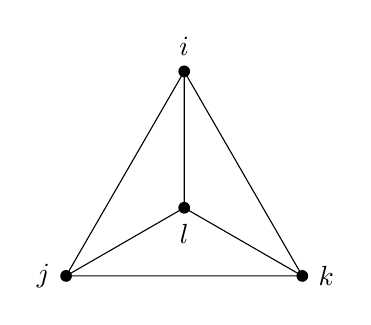
\begin{tikzpicture}[scale=1.5]
            \draw (0,-0.423) node[black,fill=black,circle,inner sep=1.5pt,label=below:$l$]{};
            \draw (-1,-1) node[black,fill=black,circle,inner sep=1.5pt,label=left:$j$]{};
            \draw (1,-1) node[black,fill=black,circle,inner sep=1.5pt,label=right:$k$]{};
            \draw (0,0.732) node[black,fill=black,circle,inner sep=1.5pt,label=$i$]{};
            \draw (0,-0.423) -- (-1,-1) -- (1,-1) -- (0,-0.423) -- (0,0.732) -- (-1,-1);
            \draw (1,-1) -- (0,0.732);
        \end{tikzpicture}
        \caption{Štiri točke, ki ne tvorijo konveksnega štirikotnika.}
        \label{fig:happy}
    \end{figure}

Izrek \ref{izrek:happyend} je osnovni rezultat, povezan s problemom, znanim 
kot ``The Happy End Problem''. Več o tem se nahaja v \cite[poglavje 29]{color}.

\section{Meje za Ramseyeva števila}

\hspace{\parindent}V tem razdelku dokažemo nekaj zgornjih in spodnjih mej za Ramseyeva števila.

\begin{trditev}
    Naj bosta $a_1,a_2 \ge 2$. Velja
    \[
        R(a_1, a_2; 2) \le \binom{a_1 + a_2 -2}{a_1-1}.
    \]
\end{trditev}

\begin{dokaz}
    Uporabimo indukcijo. Velja
    \[
        R(a_1, 2; 2) = a_1 = \binom{a_1+2-2}{a_1-1}
    \]
    in podobno za $R(2,a_2; 2)$. Direktno iz dokaza 
    izreka \ref{izrek:ramsey} sledi
    \begin{equation}
        R(a_1, a_2; r) \le R(R(a_1-1,a_2;r), R(a_1,a_2-1;r);r-1) + 1.
        \label{eq:meja}
    \end{equation}
    Za dokaz indukcijskega koraka nazadnje upoštevamo še $R(a_1,a_2;1) = a_1 + a_2 - 1$ in dobimo
    \begin{align*}
        R(a_1, a_2; 2) &\overset{\eqref{eq:meja}}{\le} R(R(a_1-1,a_2;2), R(a_1,a_2-1;2);1) +1\\
        &= (R(a_1-1,a_2;2) + R(a_1,a_2-1; 2) - 1) + 1 \\
        &\overset{{\text{IP}}}{\le} \binom{a_1 + a_2 -3}{a_1-2} + \binom{a_1 + a_2 -3}{a_1-1} \\
        &=\binom{a_1+a_2-2}{a_1-1},
    \end{align*}
    kjer zadnja enakost velja zaradi rekurzivne formule za binomski koeficient. \hfill $\blacksquare$
\end{dokaz} 

\begin{izrek}
    Naj bosta $k$ in $n$ takšni naravni števili, da velja 
    $\binom{n}{k}2^{1-\binom{k}{2}} < 1$. Potem velja 
    $R(k,k) > n$.
\end{izrek}

\begin{dokaz}
    Zadošča dokazati, da obstaja barvanje povezav $K_n$ z dvema barvama
    brez monokromatičnega $K_k$.

    Povezave grafa $K_n$ pobarvamo naključno. Vsako povezavo 
    neodvisno, z verjetnostjo $1/2$ pobarvamo s prvo barvo in 
    verjetnostjo $1/2$ z drugo barvo.
    
    V $K_n$ imamo $\binom{n}{k}$ kopij $K_k$. Naj bo $A_i$ dogodek, da 
    je $i$-ti $K_k$ monokromatičen. Velja
    \[
        \mathbb{P}(A_i) = 2 \cdot \left(\frac{1}{2}\right)^{\binom{k}{2}} = 
        2^{1-\binom{k}{2}}.
    \]
    Torej je verjetnost, da obstaja monokromatičen $K_k$, enaka 
    \[
        \mathbb{P}\left(\cup_iA_i\right) = \binom{n}{k}2^{1-\binom{k}{2}}.
    \]
    Če velja $\binom{n}{k}2^{1-\binom{k}{2}} < 1$, je verjetnost, da v 
    takšnem poljubnem barvanju ni monokromatičnega $K_k$, večja od $0$.
    Torej obstaja barvanje povezav $K_n$ z dvema barvama brez 
    monokromatičnega $K_k$. \hfill $\blacksquare$
\end{dokaz}

\begin{posledica}
    Naj bo $k \ge 3$. Potem velja $R(k, k) \ge 2^\frac{k}{2}$.
\end{posledica}

\begin{dokaz}
    Naj bo $k \ge 3$. Definiramo $n:=\floor{2^{k/2}}$. Potem
    \[
        \binom{n}{k}2^{1-\binom{k}{2}} \le
        \frac{n^k}{k!}2^{1-\frac{k(k-1)}{2}} \le 
        \left(2^{k/2}\right)^k \cdot \frac{1}{k!} \cdot 2^{1-\frac{k^2}{2}+\frac{k}{2}} =
        \frac{2^{1+\frac{k}{2}}}{k!}.
    \]
    Ker za $k \ge 3$ velja $\frac{2^{1+\frac{k}{2}}}{k!} < 1$, sledi $R(k, k) > 2^{k/2}$. \hfill $\blacksquare$
\end{dokaz}

Ta rezultat je Erdős v \cite{erdos} predstavil že leta $1947$.

Kljub obstoju tudi boljših ocen od zgornjih,
iskanje točnih vrednosti Ramseyevih števil hitro postane zelo zahtevno in 
nedosegljivo današnji tehnologiji. Tabela \ref{tab:meje} prikazuje 
trenutne znane vrednosti in meje za Ramseyeva števila $R(r, s)$. 
Razširjeno tabelo bralec najde v \cite{wiki}.

\begin{table}[H]
    \centering
    \begin{tabular}{|c||c|c|c|c|c|c|c|c|}\hline
    $R(r,s)$ & 3 & 4  & 5     & 6     & 7     & 8     & 9       & 10     \\\hline \hline
    3 & 6 & 9  & 14    & 18    & 23    & 28    & 36      & 40-41  \\\hline
    4 &   & 18 & 25    & 36-40 & 49-58 & 59-79 & 73-105 & 92-135 \\\hline
    5 &   &    & 43-46 & 59-85 & 80-133 & 101-193 & 133-282 & 149-381\\\hline
    \end{tabular}
    \caption{Znane vrednosti/meje za Ramseyeva števila $R(r, s)$.}
    \label{tab:meje}
\end{table}

Najnovejša sprememba v tabeli se je zgodila decembra leta $2023$, ko je bil objavljen 
članek, v katerem je pokazano $R(3, 10) \le 41$. 
O tem rezultatu govori \cite{r41}.

Vidimo, da je v resnici znanih zelo malo Ramseyevih števil. Če želimo dokazati, 
da je $R(s, t) = N$, moramo najti ustrezno barvanje povezav grafa $K_{N-1}$ in pokazati, da 
vsa barvanja povezav grafa $K_{N}$ ustrezajo nekemu pogoju. V teoriji bi lahko uporabili računalnik 
in preverili vsa možna barvanja za zaporedne $n$, dokler ne najdemo prvega $N$, pri katerem vsako 
barvanje zadošča zahtevanemu pogoju. Že v primeru dveh barv postane število barvanj zelo hitro 
nepredstavljivo veliko. V primeru, ko imamo več kot dve barvi ali pa v primeru $R(s, t; r)$, kjer $r > 2$, je znanega še
veliko manj. 

\begin{primer}
    Slika \ref{fig:r44} prikazuje barvanje, ki določi strogo spodnjo 
    mejo za $R(4,4)$. 
    \begin{figure}[h!]
        \centering
        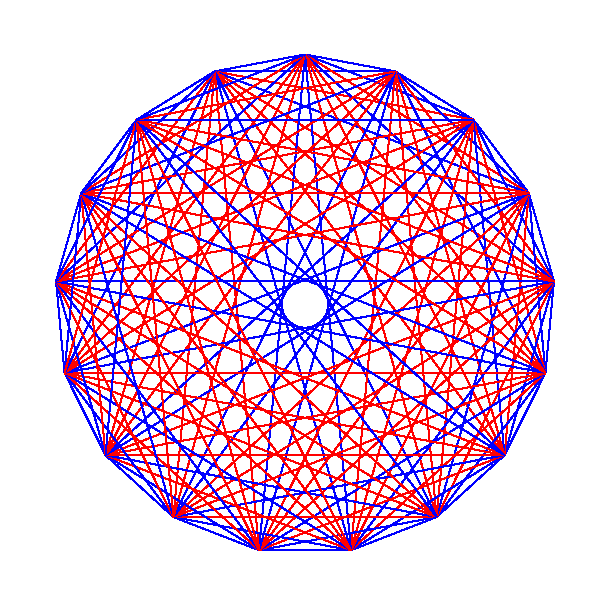
\includegraphics[scale=0.4]{r44.jpg}
        \caption{Barvanje $K_{17}$ z dvema barvama, ki ne vsebuje monokromatičnega $K_4$. Vir: \cite{r44}}
        \label{fig:r44}
    \end{figure}
\end{primer}


\section{Grafovska Ramseyeva števila}

\begin{definicija}
    Naj bodo $G_1, \dots, G_k$ enostavni grafi. \emph{Grafovsko Ramseyevo število}
    $R(G_1, G_2, \dots, G_k)$ je najmanjše naravno število $n$, za katerega velja, da 
    vsako barvanje s $k$ barvami povezav $K_n$ vsebuje $G_i$ barve $i$ za nek $i$. 
\end{definicija}

Obstoj Grafovskega Ramseyevega števila sledi direktno iz izreka \ref{izrek:ramsey}.

\begin{zgled}
    Določimo $R(P_4, C_4)$.
    %\textit{Opomba o oznakah:} $P_n$ označuje pot na $n$ vozliščih, $C_n$ pa cikel na $n$ vozliščih.
    Slika \ref{fig:p4c4} prikazuje barvanje, ki ne vsebuje niti $C_4$ rdeče 
    barve niti $P_4$ modre barve. Sledi $R(P_4,C_4) > 4$.

    \begin{figure}[h!]
        \centering
        \newcommand\size{1}
        \begin{tikzpicture}[scale=2]
            \draw[thick,red] (45:\size) \foreach \a in {45,135,225} { -- (\a:\size) } -- cycle;
            \draw[thick,blue]  (225:\size) \foreach \a in {225,315,45} { -- (\a:\size) };
            \draw[thick,blue]  (135:\size) \foreach \a in {135,315} { -- (\a:\size) };
            \foreach \a in {45,135,225,315} { \node[black,fill=black,circle,inner sep=1.5pt] at (\a:\size){}; }
        \end{tikzpicture}
        \caption{Barvanje $K_{4}$ z dvema barvama, ki ne vsebuje niti $C_4$ rdeče 
        barve niti $P_4$ modre barve.}
        \label{fig:p4c4}
    \end{figure}

    Pokažimo, da je $R(P_4, C_4) \le 5$. Naj bodo $\set{v_0, v_1, v_2, v_3, v_4}$ vozlišča
    $K_5$, katerega povezave pobarvamo z rdečo in modro barvo.
    \begin{itemize}
        \item Recimo, da je $v_0$ v vsaj dveh povezavah modre barve -- $v_0v_1$ in $v_0v_2$. Če je
        katera od povezav $v_1v_3, v_1v_4, v_2v_3, v_2v_4$ modra, imamo $P_4$ modre barve.
        Sicer imamo rdeč $C_4$.

        \item Recimo, da je $v_0$ v vsaj treh povezavah rdeče barve. Naj bodo to $v_0v_1$, $v_0v_2$
        in $v_0v_3$. Če sta vsaj dve povezavi med $v_1$, $v_2$ in $v_3$ rdeči, imamo 
        rdeč $C_4$. Recimo, da je kvečjemu ena rdeča in brez škode za splošnost $v_1v_2$ in $v_2v_3$ 
        modri. Če je $v_1v_4$ ali $v_1v_4$ modra, imamo moder $P_4$, sicer imamo rdeč $C_4$.
    \end{itemize}

    Dokazali smo, da velja $R(P_4, C_4) = R(P_4, P_4) = 5$.
\end{zgled}

Naslednji izrek je leta $1977$ dokazal Chvátal.

\begin{izrek}[Chvátal]
    Naj bo $T$ drevo na $m$ vozliščih. Dokažite, da je $R(T, K_n) = (m-1)(n-1)+1$.    
\end{izrek}

\begin{dokaz}
    Za dokaz spodnje meje pobarvamo graf $K_{(m-1)(n-1)}$ tako, da bo rdeč del enak 
    $(n-1)K_{m-1}$ (torej imamo $n-1$ disjunktnih rdečih grafov $K_{m-1}$). Rdeče povezane komponente 
    bodo tedaj velikosti $m-1$, torej graf ne vsebuje rdečega drevesa velikosti $m$. Poln moder 
    podgraf lahko vsebuje kvečjemu eno povezavo iz vsakega disjunktnega $K_{m-1}$, torej je 
    velikosti kvečjemu $n-1$.

    Zgornjo mejo dokažemo z indukcijo na $n$, pri čemer si pomagamo z naslednjo znano lemo.
    \begin{lema*}
        Naj bo $m \ge 2$. Če je $H$ graf z minimalno stopnjo vsaj $m-1$, potem vsebuje vsako drevo na $m$ vozliščih.
    \end{lema*}
    \begin{dokaz}
        Lemo dokažemo s pomočjo indukcije na $m$. V primeru $m=2$ je pogoj izpolnjen. Naj bo 
        $T$ drevo na $m > 2$ vozliščih in predpostavimo, da lema velja za $m-1$. Naj bo $H$ 
        graf z minimalno stopnjo vsaj $m-1$ in $T$ drevo na $m$ vozliščih. Naj bo $v$ list drevesa. 
        Tedaj $H$ vsebuje $S = T - u$. Velja $\abs{S} = {m-1}$, torej je vsako vozlišče 
        $v \in S$ povezano s kakšnim vozliščem, ki ni vsebovano v $S$. Posledično lahko 
        priključimo takšno vozlišče, da dobimo $T$. \hfill $\blacksquare$
    \end{dokaz}
    Naj bo $n = 1$. Potem za moder $K_1$ ne potrebujemo nobene povezave in je pogoj izpolnjen. 
    Naj bo sedaj $n > 1$. Predpostavimo, da pogoj naloge velja za $n - 1$. Recimo, da imamo neko barvanje povezav grafa $K_{(m-1)(n-1)+1}$ z dvema barvama. 
    \begin{itemize}
        \item Naj bo $v$ poljubno vozlišče. Če ima $v$ več kot $(m-1)(n-2)$ modrih povezav, potem med temi sosedi 
        po indukcijski predpostavki obstaja bodisi rdeč $T$ bodisi moder $K_{n-1}$. V slednjem 
        primeru skupaj z vozliščem $v$ dobimo $K_n$, sicer pa že imamo rdeč $T$.
        \item Recimo, da ima vsako vozlišče kvečjemu $(m-1)(n-2)$ modrih povezav in posledično 
        vsaj $m-1$ rdečih povezav. V tem primeru nam zgornja lema zagotovi rdeč $T$. Pri tem 
        moramo paziti samo na primer $m = 1$, vendar v tem primeru ponovno ne potrebujemo 
        nobene povezave, da je pogoj izpolnjen.
    \end{itemize}
    Zagotovo se bo zgodila ena od teh dveh možnosti, torej smo končali.  \hfill $\blacksquare$
\end{dokaz}


\section{Schurova števila}

\begin{izrek}[Schur] \label{izrek:schur}
    Za vsako naravno število $k$ obstaja takšno naravno število $n$, da za vsako 
    $k$-barvanje elementov množice $\set{1, 2, \dots, n}$ obstajajo števila $x$, $y$ in $z$
    iz $\set{1, 2, \dots, n}$ iste barve z lastnostjo $x + y = z$.
\end{izrek}

\begin{dokaz}
    Naj bo $k$ naravno število in $n = R_k(3, \dots, 3) := R(\underbrace{3, \dots, 3}_{\text{$k$-krat}})$.
    
    Naj bo množica $\set{1, 2, \dots, n}$ pobarvana s $k$ barvami. 
    Torej imamo particijo
    \[
        \set{1, 2, \dots, n} = S_1 \cup S_2 \cup \dotsb \cup S_k,
    \]
    kjer $S_i$ vsebuje natanko tiste elemente, ki so pobarvani z $i$-to barvo.

    Konstruirajmo poln graf $G$ na $n+1$ vozliščih, ki jih označimo z
    $1, 2, \dots, n+1$. Naj bo povezava, ki vsebuje $i$ in $j$, takšne barve $r$,
    da velja $\abs{i-j} \in S_r$. 

    Ker velja $n+1 > n = R_k(3, \dots, 3)$, graf $G$ vsebuje monokromatičen 
    trikotnik. Torej obstajajo $i, j, k \in \set{1,2, \dots, n+1}$, za katere 
    velja, da so $\abs{i-j}$, $\abs{j-k}$ in $\abs{k-i}$ iste barve. Brez škode 
    za splošnost naj bo $i > j > k$. Naj bo $x = \abs{i - j}$, $y = \abs{j - k}$ in 
    $z = {k - i}$. Res velja
    \[
        x + y = i - j + j - k = \abs{k - i} = z,
    \]
    kjer so $x$, $y$ in $z$ iz $\set{1, 2, \dots, n}$. \hfill $\blacksquare$
\end{dokaz}

\begin{definicija}
    Naj bo $k$ naravno število. Najmanjše takšno število $n$, ki zadošča 
    pogoju iz izreka \ref{izrek:schur}, se imenuje 
    $k$-to \emph{Schurovo število}.
\end{definicija}

Trenutno je znanih samo prvih pet Schurovih števil. Zaporedoma so $2$, $5$,
$14$, $45$ in $161$. Dokaz, da je $S(5) = 161$ iz leta $2017$ je znan največji 
matematični dokaz v smislu porabljenega prostora -- potrebna sta bila 
kar dva petabajta podatkov. Problem je bil odprt več kot stoletje, več 
o dokazu pa se nahaja v \cite{schur}.

\section{Zaključek}
\hspace{\parindent}Ramseyeva teorija je še vedno zelo aktualno področje, v 
katerem letno prihaja do novih spoznanj. 
V članku smo predstavili nekaj osnovnih pojmov in rezultatov.

\begin{thebibliography}{99}
    \bibitem{r41} V.~Angeltveit, \emph{R(3,10) <= 41}, 2024, arXiv:2401.00392 [math.CO].
    \bibitem{erdos} P.~Erdös. \emph{Some Remarks on the Theory of Graphs}. Bulletin of the
    American Mathematical Society, 53(4):292-294, 1947.
    \bibitem{schur} M.~J.~H.~Heule, \emph{Schur Number Five}, 2017, arXiv:1711.08076 [cs.LO].
    \bibitem{color} A.~Soifer, \emph{The Mathematical Coloring Book: Mathematics of Coloring and the Colorful Life of its Creators},
    Springer, 2009.
    \bibitem{west} D.~B.~West, \emph{Introduction to Graph Theory}, Prentice Hall, 2001.
    \bibitem{r44} \emph{Breakthrough in Ramsey theory}, Spletna stran: https://anthonybonato.com/breakthrough-in-ramsey-theory, ogled 17. 3. 2025.
    \bibitem{r333} \emph{Clebsch graph}, Wikipedia, Spletna stran: https://en.wikipedia.org/wiki/Clebsch\_graph, ogled 29.~1.~2025.
    \bibitem{wiki} \emph{Ramsey's theorem}, Wipedia, Spletna stran: https://en.wikipedia.org/wiki/Ramsey's\_theorem, ogled: 28.~1.~2025.
\end{thebibliography}

\end{document}